% Graphic for TeX using PGF
% Title: /home/guillaume/Documents/Université de Montréal/Automne 2014/Génie logiciel/Devoir/devoir-3/diagramme-de-classes-changement-2.dia
% Creator: Dia v0.97.3
% CreationDate: Sat Dec  6 12:51:34 2014
% For: guillaume
% \usepackage{tikz}
% The following commands are not supported in PSTricks at present
% We define them conditionally, so when they are implemented,
% this pgf file will use them.
\ifx\du\undefined
  \newlength{\du}
\fi
\setlength{\du}{15\unitlength}
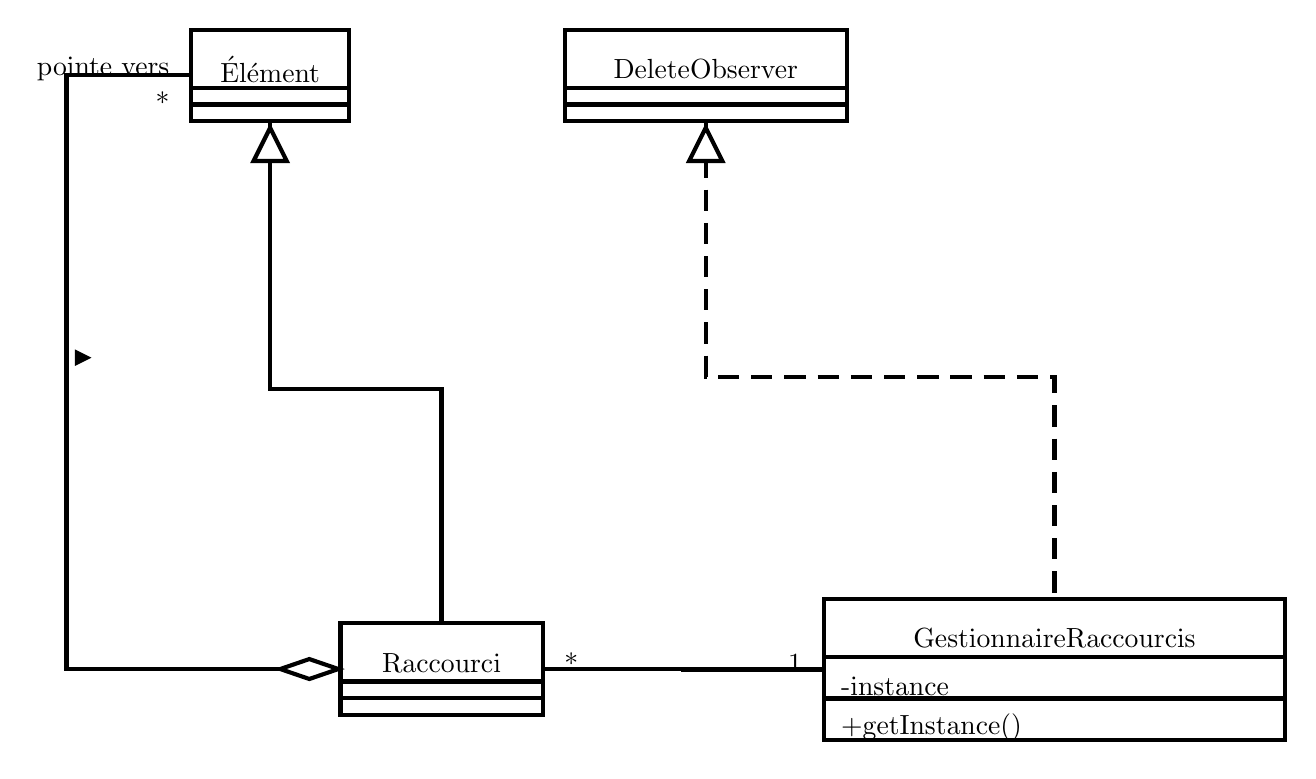
\begin{tikzpicture}
\pgftransformxscale{1.000000}
\pgftransformyscale{-1.000000}
\definecolor{dialinecolor}{rgb}{0.000000, 0.000000, 0.000000}
\pgfsetstrokecolor{dialinecolor}
\definecolor{dialinecolor}{rgb}{1.000000, 1.000000, 1.000000}
\pgfsetfillcolor{dialinecolor}
\pgfsetlinewidth{0.100000\du}
\pgfsetdash{}{0pt}
\definecolor{dialinecolor}{rgb}{1.000000, 1.000000, 1.000000}
\pgfsetfillcolor{dialinecolor}
\fill (10.309500\du,2.790000\du)--(10.309500\du,4.190000\du)--(14.122000\du,4.190000\du)--(14.122000\du,2.790000\du)--cycle;
\definecolor{dialinecolor}{rgb}{0.000000, 0.000000, 0.000000}
\pgfsetstrokecolor{dialinecolor}
\draw (10.309500\du,2.790000\du)--(10.309500\du,4.190000\du)--(14.122000\du,4.190000\du)--(14.122000\du,2.790000\du)--cycle;
% setfont left to latex
\definecolor{dialinecolor}{rgb}{0.000000, 0.000000, 0.000000}
\pgfsetstrokecolor{dialinecolor}
\node at (12.215750\du,3.740000\du){Élément};
\definecolor{dialinecolor}{rgb}{1.000000, 1.000000, 1.000000}
\pgfsetfillcolor{dialinecolor}
\fill (10.309500\du,4.190000\du)--(10.309500\du,4.590000\du)--(14.122000\du,4.590000\du)--(14.122000\du,4.190000\du)--cycle;
\definecolor{dialinecolor}{rgb}{0.000000, 0.000000, 0.000000}
\pgfsetstrokecolor{dialinecolor}
\draw (10.309500\du,4.190000\du)--(10.309500\du,4.590000\du)--(14.122000\du,4.590000\du)--(14.122000\du,4.190000\du)--cycle;
\definecolor{dialinecolor}{rgb}{1.000000, 1.000000, 1.000000}
\pgfsetfillcolor{dialinecolor}
\fill (10.309500\du,4.590000\du)--(10.309500\du,4.990000\du)--(14.122000\du,4.990000\du)--(14.122000\du,4.590000\du)--cycle;
\definecolor{dialinecolor}{rgb}{0.000000, 0.000000, 0.000000}
\pgfsetstrokecolor{dialinecolor}
\draw (10.309500\du,4.590000\du)--(10.309500\du,4.990000\du)--(14.122000\du,4.990000\du)--(14.122000\du,4.590000\du)--cycle;
\pgfsetlinewidth{0.100000\du}
\pgfsetdash{}{0pt}
\definecolor{dialinecolor}{rgb}{1.000000, 1.000000, 1.000000}
\pgfsetfillcolor{dialinecolor}
\fill (13.909500\du,17.090000\du)--(13.909500\du,18.490000\du)--(18.779500\du,18.490000\du)--(18.779500\du,17.090000\du)--cycle;
\definecolor{dialinecolor}{rgb}{0.000000, 0.000000, 0.000000}
\pgfsetstrokecolor{dialinecolor}
\draw (13.909500\du,17.090000\du)--(13.909500\du,18.490000\du)--(18.779500\du,18.490000\du)--(18.779500\du,17.090000\du)--cycle;
% setfont left to latex
\definecolor{dialinecolor}{rgb}{0.000000, 0.000000, 0.000000}
\pgfsetstrokecolor{dialinecolor}
\node at (16.344500\du,18.040000\du){Raccourci};
\definecolor{dialinecolor}{rgb}{1.000000, 1.000000, 1.000000}
\pgfsetfillcolor{dialinecolor}
\fill (13.909500\du,18.490000\du)--(13.909500\du,18.890000\du)--(18.779500\du,18.890000\du)--(18.779500\du,18.490000\du)--cycle;
\definecolor{dialinecolor}{rgb}{0.000000, 0.000000, 0.000000}
\pgfsetstrokecolor{dialinecolor}
\draw (13.909500\du,18.490000\du)--(13.909500\du,18.890000\du)--(18.779500\du,18.890000\du)--(18.779500\du,18.490000\du)--cycle;
\definecolor{dialinecolor}{rgb}{1.000000, 1.000000, 1.000000}
\pgfsetfillcolor{dialinecolor}
\fill (13.909500\du,18.890000\du)--(13.909500\du,19.290000\du)--(18.779500\du,19.290000\du)--(18.779500\du,18.890000\du)--cycle;
\definecolor{dialinecolor}{rgb}{0.000000, 0.000000, 0.000000}
\pgfsetstrokecolor{dialinecolor}
\draw (13.909500\du,18.890000\du)--(13.909500\du,19.290000\du)--(18.779500\du,19.290000\du)--(18.779500\du,18.890000\du)--cycle;
\pgfsetlinewidth{0.100000\du}
\pgfsetdash{}{0pt}
\pgfsetmiterjoin
\pgfsetbuttcap
{
\definecolor{dialinecolor}{rgb}{0.000000, 0.000000, 0.000000}
\pgfsetfillcolor{dialinecolor}
% was here!!!
\definecolor{dialinecolor}{rgb}{0.000000, 0.000000, 0.000000}
\pgfsetstrokecolor{dialinecolor}
\draw (13.859657\du,18.190000\du)--(7.309510\du,18.190000\du)--(7.309510\du,3.890000\du)--(10.259722\du,3.890000\du);
}
\definecolor{dialinecolor}{rgb}{0.000000, 0.000000, 0.000000}
\pgfsetstrokecolor{dialinecolor}
\draw (12.601079\du,18.190000\du)--(7.309510\du,18.190000\du)--(7.309510\du,3.890000\du)--(10.259722\du,3.890000\du);
\pgfsetdash{}{0pt}
\pgfsetmiterjoin
\pgfsetbuttcap
\definecolor{dialinecolor}{rgb}{1.000000, 1.000000, 1.000000}
\pgfsetfillcolor{dialinecolor}
\fill (13.859657\du,18.190000\du)--(13.159657\du,18.430000\du)--(12.459657\du,18.190000\du)--(13.159657\du,17.950000\du)--cycle;
\pgfsetlinewidth{0.100000\du}
\pgfsetdash{}{0pt}
\pgfsetmiterjoin
\pgfsetbuttcap
\definecolor{dialinecolor}{rgb}{0.000000, 0.000000, 0.000000}
\pgfsetstrokecolor{dialinecolor}
\draw (13.859657\du,18.190000\du)--(13.159657\du,18.430000\du)--(12.459657\du,18.190000\du)--(13.159657\du,17.950000\du)--cycle;
% setfont left to latex
\definecolor{dialinecolor}{rgb}{0.000000, 0.000000, 0.000000}
\pgfsetstrokecolor{dialinecolor}
\node[anchor=west] at (7.409510\du,10.890000\du){};
\definecolor{dialinecolor}{rgb}{0.000000, 0.000000, 0.000000}
\pgfsetfillcolor{dialinecolor}
\fill (7.509510\du,10.890000\du)--(7.509510\du,10.490000\du)--(7.909510\du,10.690000\du)--cycle;
\definecolor{dialinecolor}{rgb}{0.000000, 0.000000, 0.000000}
\pgfsetstrokecolor{dialinecolor}
\node[anchor=east] at (12.259657\du,18.040000\du){};
\definecolor{dialinecolor}{rgb}{0.000000, 0.000000, 0.000000}
\pgfsetstrokecolor{dialinecolor}
\node[anchor=east] at (10.059722\du,3.740000\du){ pointe vers};
\definecolor{dialinecolor}{rgb}{0.000000, 0.000000, 0.000000}
\pgfsetstrokecolor{dialinecolor}
\node[anchor=east] at (10.059722\du,4.540000\du){*};
\pgfsetlinewidth{0.100000\du}
\pgfsetdash{}{0pt}
\pgfsetmiterjoin
\pgfsetbuttcap
{
\definecolor{dialinecolor}{rgb}{0.000000, 0.000000, 0.000000}
\pgfsetfillcolor{dialinecolor}
% was here!!!
\definecolor{dialinecolor}{rgb}{0.000000, 0.000000, 0.000000}
\pgfsetstrokecolor{dialinecolor}
\draw (12.215750\du,5.040281\du)--(12.215750\du,11.440000\du)--(16.344500\du,11.440000\du)--(16.344500\du,17.039719\du);
}
\definecolor{dialinecolor}{rgb}{0.000000, 0.000000, 0.000000}
\pgfsetstrokecolor{dialinecolor}
\draw (12.215750\du,5.952084\du)--(12.215750\du,11.440000\du)--(16.344500\du,11.440000\du)--(16.344500\du,17.039719\du);
\pgfsetmiterjoin
\definecolor{dialinecolor}{rgb}{1.000000, 1.000000, 1.000000}
\pgfsetfillcolor{dialinecolor}
\fill (12.615750\du,5.952084\du)--(12.215750\du,5.152084\du)--(11.815750\du,5.952084\du)--cycle;
\pgfsetlinewidth{0.100000\du}
\pgfsetdash{}{0pt}
\pgfsetmiterjoin
\definecolor{dialinecolor}{rgb}{0.000000, 0.000000, 0.000000}
\pgfsetstrokecolor{dialinecolor}
\draw (12.615750\du,5.952084\du)--(12.215750\du,5.152084\du)--(11.815750\du,5.952084\du)--cycle;
% setfont left to latex
\pgfsetlinewidth{0.100000\du}
\pgfsetdash{}{0pt}
\definecolor{dialinecolor}{rgb}{1.000000, 1.000000, 1.000000}
\pgfsetfillcolor{dialinecolor}
\fill (19.309500\du,2.790000\du)--(19.309500\du,4.190000\du)--(26.109500\du,4.190000\du)--(26.109500\du,2.790000\du)--cycle;
\definecolor{dialinecolor}{rgb}{0.000000, 0.000000, 0.000000}
\pgfsetstrokecolor{dialinecolor}
\draw (19.309500\du,2.790000\du)--(19.309500\du,4.190000\du)--(26.109500\du,4.190000\du)--(26.109500\du,2.790000\du)--cycle;
% setfont left to latex
\definecolor{dialinecolor}{rgb}{0.000000, 0.000000, 0.000000}
\pgfsetstrokecolor{dialinecolor}
\node at (22.709500\du,3.740000\du){DeleteObserver};
\definecolor{dialinecolor}{rgb}{1.000000, 1.000000, 1.000000}
\pgfsetfillcolor{dialinecolor}
\fill (19.309500\du,4.190000\du)--(19.309500\du,4.590000\du)--(26.109500\du,4.590000\du)--(26.109500\du,4.190000\du)--cycle;
\definecolor{dialinecolor}{rgb}{0.000000, 0.000000, 0.000000}
\pgfsetstrokecolor{dialinecolor}
\draw (19.309500\du,4.190000\du)--(19.309500\du,4.590000\du)--(26.109500\du,4.590000\du)--(26.109500\du,4.190000\du)--cycle;
\definecolor{dialinecolor}{rgb}{1.000000, 1.000000, 1.000000}
\pgfsetfillcolor{dialinecolor}
\fill (19.309500\du,4.590000\du)--(19.309500\du,4.990000\du)--(26.109500\du,4.990000\du)--(26.109500\du,4.590000\du)--cycle;
\definecolor{dialinecolor}{rgb}{0.000000, 0.000000, 0.000000}
\pgfsetstrokecolor{dialinecolor}
\draw (19.309500\du,4.590000\du)--(19.309500\du,4.990000\du)--(26.109500\du,4.990000\du)--(26.109500\du,4.590000\du)--cycle;
\pgfsetlinewidth{0.100000\du}
\pgfsetdash{{1.000000\du}{1.000000\du}}{0\du}
\pgfsetdash{{0.400000\du}{0.400000\du}}{0\du}
\pgfsetmiterjoin
\pgfsetbuttcap
{
\definecolor{dialinecolor}{rgb}{0.000000, 0.000000, 0.000000}
\pgfsetfillcolor{dialinecolor}
% was here!!!
\definecolor{dialinecolor}{rgb}{0.000000, 0.000000, 0.000000}
\pgfsetstrokecolor{dialinecolor}
\draw (22.709500\du,5.040281\du)--(22.709500\du,11.144927\du)--(31.110000\du,11.144927\du)--(31.110000\du,16.449573\du);
}
\definecolor{dialinecolor}{rgb}{0.000000, 0.000000, 0.000000}
\pgfsetstrokecolor{dialinecolor}
\draw (22.709500\du,5.952084\du)--(22.709500\du,11.144927\du)--(31.110000\du,11.144927\du)--(31.110000\du,16.449573\du);
\pgfsetmiterjoin
\definecolor{dialinecolor}{rgb}{1.000000, 1.000000, 1.000000}
\pgfsetfillcolor{dialinecolor}
\fill (23.109500\du,5.952084\du)--(22.709500\du,5.152084\du)--(22.309500\du,5.952084\du)--cycle;
\pgfsetlinewidth{0.100000\du}
\pgfsetdash{}{0pt}
\pgfsetmiterjoin
\definecolor{dialinecolor}{rgb}{0.000000, 0.000000, 0.000000}
\pgfsetstrokecolor{dialinecolor}
\draw (23.109500\du,5.952084\du)--(22.709500\du,5.152084\du)--(22.309500\du,5.952084\du)--cycle;
% setfont left to latex
\pgfsetlinewidth{0.100000\du}
\pgfsetdash{}{0pt}
\definecolor{dialinecolor}{rgb}{1.000000, 1.000000, 1.000000}
\pgfsetfillcolor{dialinecolor}
\fill (25.550000\du,16.500000\du)--(25.550000\du,17.900000\du)--(36.670000\du,17.900000\du)--(36.670000\du,16.500000\du)--cycle;
\definecolor{dialinecolor}{rgb}{0.000000, 0.000000, 0.000000}
\pgfsetstrokecolor{dialinecolor}
\draw (25.550000\du,16.500000\du)--(25.550000\du,17.900000\du)--(36.670000\du,17.900000\du)--(36.670000\du,16.500000\du)--cycle;
% setfont left to latex
\definecolor{dialinecolor}{rgb}{0.000000, 0.000000, 0.000000}
\pgfsetstrokecolor{dialinecolor}
\node at (31.110000\du,17.450000\du){GestionnaireRaccourcis};
\definecolor{dialinecolor}{rgb}{1.000000, 1.000000, 1.000000}
\pgfsetfillcolor{dialinecolor}
\fill (25.550000\du,17.900000\du)--(25.550000\du,18.900000\du)--(36.670000\du,18.900000\du)--(36.670000\du,17.900000\du)--cycle;
\definecolor{dialinecolor}{rgb}{0.000000, 0.000000, 0.000000}
\pgfsetstrokecolor{dialinecolor}
\draw (25.550000\du,17.900000\du)--(25.550000\du,18.900000\du)--(36.670000\du,18.900000\du)--(36.670000\du,17.900000\du)--cycle;
% setfont left to latex
\definecolor{dialinecolor}{rgb}{0.000000, 0.000000, 0.000000}
\pgfsetstrokecolor{dialinecolor}
\node[anchor=west] at (25.700000\du,18.600000\du){-instance};
\definecolor{dialinecolor}{rgb}{1.000000, 1.000000, 1.000000}
\pgfsetfillcolor{dialinecolor}
\fill (25.550000\du,18.900000\du)--(25.550000\du,19.900000\du)--(36.670000\du,19.900000\du)--(36.670000\du,18.900000\du)--cycle;
\definecolor{dialinecolor}{rgb}{0.000000, 0.000000, 0.000000}
\pgfsetstrokecolor{dialinecolor}
\draw (25.550000\du,18.900000\du)--(25.550000\du,19.900000\du)--(36.670000\du,19.900000\du)--(36.670000\du,18.900000\du)--cycle;
% setfont left to latex
\definecolor{dialinecolor}{rgb}{0.000000, 0.000000, 0.000000}
\pgfsetstrokecolor{dialinecolor}
\node[anchor=west] at (25.700000\du,19.600000\du){+getInstance()};
\pgfsetlinewidth{0.100000\du}
\pgfsetdash{}{0pt}
\pgfsetmiterjoin
\pgfsetbuttcap
{
\definecolor{dialinecolor}{rgb}{0.000000, 0.000000, 0.000000}
\pgfsetfillcolor{dialinecolor}
% was here!!!
\definecolor{dialinecolor}{rgb}{0.000000, 0.000000, 0.000000}
\pgfsetstrokecolor{dialinecolor}
\draw (18.829803\du,18.190000\du)--(22.164730\du,18.190000\du)--(22.164730\du,18.200000\du)--(25.499658\du,18.200000\du);
}
% setfont left to latex
\definecolor{dialinecolor}{rgb}{0.000000, 0.000000, 0.000000}
\pgfsetstrokecolor{dialinecolor}
\node[anchor=west] at (22.264730\du,18.045000\du){};
\definecolor{dialinecolor}{rgb}{0.000000, 0.000000, 0.000000}
\pgfsetstrokecolor{dialinecolor}
\node[anchor=west] at (19.029803\du,18.040000\du){*};
\definecolor{dialinecolor}{rgb}{0.000000, 0.000000, 0.000000}
\pgfsetstrokecolor{dialinecolor}
\node[anchor=east] at (25.299658\du,18.050000\du){1};
\end{tikzpicture}
